\documentclass{llncs}
%
\usepackage{makeidx}  % allows for indexgeneration
\usepackage[british]{babel}
\usepackage{url}
\usepackage[pdftex,colorlinks=true]{hyperref}
\usepackage{graphicx}
%\fussy


\title{Dear CAV, We Need to Talk About Reproducibility}

\author{Tom Crick\inst{1} \and Benjamin A. Hall\inst{2} \and Samin Ishtiaq\inst{3}}

\institute{Department of Computing \& Information Systems\\Cardiff Metropolitan University, UK\\
\email{tcrick@cardiffmet.ac.uk}
\and
MRC Cancer Unit, University of Cambridge, UK\\
\email{bh418@mrc-cu.cam.ac.uk}
\and
Microsoft Research Cambridge, UK\\
\email{samin.ishtiaq@microsoft.com}
}

\raggedbottom
\begin{document}
%
\frontmatter          % for the preliminaries
%
\pagestyle{headings}  % switches on printing of running heads
%\addtocmark{} % additional mark in the TOC

\maketitle

\begin{abstract}

How many times have you tried to re-implement a past CAV tool paper, and failed?

Reliably reproducing published scientific discoveries has been
acknowledged as a barrier to scientific progress for some time but there remains only a small subset of software available to
support the specific needs of the research community (i.e. beyond
generic tools such as source code repositories). In this paper we
propose an infrastructure for enabling
reproducibility in the our community, by automating the
build, unit testing and benchmarking of research software. 

We propose a workflow model to adopt for promoting and embedding reproducibility
into future instances of CAV, illustrated by a case study using the
BioModelAnalyzer software.
\end{abstract}

% TO DO:
% consistency of artefact (UK) vs. artifact (US)...
% missing refs
% trim to six pages!

\section{Introduction}\label{intro}

\begin{quotation}
{\emph{CAV 2015 is the 27th in a series dedicated to the advancement
    of the theory and practice of computer-aided formal analysis
    methods for hardware and software systems.  CAV considers it vital
    to continue spurring advances in hardware and software
    verification while expanding to new domains such as biological
    systems and computer security. The conference covers the spectrum
    from theoretical results to concrete applications, with an
    emphasis on practical verification tools and the algorithms and
    techniques that are needed for their implementation.}}
\end{quotation}
 
This is not a theory paper or a tool paper, nor an industrial case
study. The aim of this paper is to start a discussion in the CAV
community about reproducibility of algorithms, models, tools and
benchmarks across the computer-aided formal analysis and verification
research domain. There is a significant opportunity for the CAV
community to identify and address the technical and socio-cultural
issues surrounding reproducibility in both the cognate research domain
as well as more broadly for computing science; a desirable outcome
would be a clear specification to encourage, enable and enforce
reproducibility. Expressing a standard for reproducibility would have
a clear benefit for researchers as well as the CAV community as a
whole.

The reproducibility of scientific discovery has become a major topic
of discussion over the past few years, as we have seen a step-change
in how science and engineering is done. Experiments, simulations,
models, benchmarks, even proofs cannot be done without leveraging
software and computation. A 2012 report by the Royal Society stated
that computational techniques have ``{\emph{moved on from assisting
scientists in doing science, to transforming both how science is done
and what science is done}}''~\cite{rssaaoe:2012}. Following a
revolution in the sharing and dissemination of published papers
(\emph{open access}) and the subsequent discussions relating to the
sharing of protocols and materials (\emph{open science}) the ability
of a researcher to take published results and data and reimplement the
described workflow has been under significant
scrutiny~\cite{stodden-et-al:2013,sandve-et-al:2013,wilson-et-al:2014}. This
has been further supported by wider cultural changes in the scientific
community, where increasingly high profile -- and irreproducible --
results are being identified and retracted from the
literature\footnote{Retraction Watch: Tracking retractions as a window
into the scientific
process\\\url{http://retractionwatch.com/}}. Alongside the
ramifications of damaging the credibility and veracity of the research
base, there are also clear consequences for research funding: recent statistics
for US National Institute of Health funding between 1992 and 2012
found that papers retracted due to misconduct accounted for
approximately \$58 million, c.\$400,000 per
paper~\cite{stern-et-al:2014}. We have previously documented some of
the technical and cultural barriers to reproducing work across
computing and computational sciences, both in terms of the sharing of
algorithms~\cite{crick-et-al_recomp2014} and models and benchmark
sets~\cite{crick-et-al_wssspe2}. Nevertheless, the impact of
irreproducibility is keenly felt across multiple disciplines, with
well discussed issues in computer science~\cite{collberg-et-al:2014},
life sciences~\cite{rollins-et-al:2014},
psychology~\cite{chambers-et-al:2014} and the social
sciences~\cite{conte-et-al:2012}.

While reproducibility has been acknowledged as a desirable quality --
including at CAV through the CAV Artefact
Evaluation\footnote{\url{http://i-cav.org/2015/evaluation/}} process
-- and driven at a number of conferences and workshops by the cTuning
and Collective Mind initiatives\footnote{\url{http://ctuning.org/}}
e.g. CGO\footnote{\url{http://ctuning.org/cm/wiki/index.php?title=Reproducibility:AE:CGO2015}},
PPoPP\footnote{\url{http://ctuning.org/cm/wiki/index.php?title=Reproducibility:AE:PPoPP2015}},
TRUST\footnote{\url{http://ctuning.org/cm/wiki/index.php?title=Events:TRUST2014}}
and ADAPT\footnote{\url{http://www.adapt-workshop.org/}}, there are
still significant issues to overcome before we have a step change in
how researchers view reproduciblity as a fundamental part of the
research process.  There appear to be a focus on the community-driven
reviewing and validation of research
outputs~\cite{fursin+dubach:2014}, but most, if not all, conferences
explicitly note that the provision of \emph{artefacts} (an accessible
tool for reproducing results) is desirable but does not change the
ultimate outcome of the review e.g. SPLASH
(OOPSLA)\footnote{\url{http://2014.splashcon.org/track/splash2014-artifacts\#About}}.
Furthermore, while several journals (e.g. Bioinformatics, PLoS
Computational Biology) explicitly require that source code and data is
made available online under some form of open source license, this
static approach does little for enabling verification or validation of
scientific results at a later stage. This applies to the authors of
this paper: as we explore in section~\ref{example}, we have published
a number of times in CAV and our research and experiments would have
benefited had such a reproducibility standard (and infrastructure)
existed and been front and centre in the CAV community.

While it is encouraging that there is a consensus emerging on the
importance of reproducibility (and repeatability, recomputability and
the multitude of `Rs' that underpin e-research), it should not be a
topic only discussed at conference and workshops convened specifically
on the topic of reproducibility. The authors have been involved in
this process~\cite{crick+chuehong:2014}, but for it to progress it has
to be embraced by specific research communities at their major
conferences and workshops. Therein lies a fundamental advantage of
computer science and more broadly, computational science: the unique
ability to easily share the raw outputs of our work as software and
datafiles. As researchers in this field, we should be good at this;
ultimately, we are setting a challenge for the CAV community: we need
to explicitly state that this is important and address it or don't
bother doing it at all.

% http://2014.splashcon.org/track/splash2014-artifacts#About
% \begin{quotation}
% {\emph{{\textbf{OOPSLA Artifacts:}} The Artifact Evaluation Committee has been formed
% to assess how well paper authors prepare artifacts in support of such
% future researchers. Roughly, authors of papers who wish to participate
% are invited to submit an artifact that supports the conclusions of the
% paper. The Artifact Evaluation Committee will read the paper and
% explore the artifact to give the authors third-party feedback about
% how well the artifact supports the paper and how easy it is, in the
% committee’s opinion, for future researchers to use the artifact. This
% submission is voluntary and will not influence the final decision
% regarding the papers. Papers that go through the Artifact Evaluation
% process successfully receive a seal of approval printed on the first
% page of the paper in the OOPSLA proceedings.}}
% \end{quotation}

% TACAS\footnote{\url{http://www.etaps.org/index.php/2015/tacas}}
%Cite: Recomputation Manifesto~\cite{gent:2013}, 10 Simple Rules for Reproducible
%Research~\cite{sandve-et-al:2013}, Stodden~\cite{stodden-et-al:2013},
%changes to dissemination in other fields e.g. psychology~\cite{chambers-et-al:2014}.

% Other examples: ACM SIGPLAN TRUST~\cite{fursin+dubach:2014}; using proofs and
% Coq e.g. POPL/PLDI/ICFP.

% Q: do we need to define artefact? different from model, etc, also
% domain terminology e.g. CS vs. physics.

% However, whilst provision of a single implementation or the current
% source code may not be sufficient to satisfactorily reproduce
% computational discoveries.  As discussed
% previously~\cite{crick-et-al_recomp2014}, external dependencies may
% change the behaviour, or in the case of an incompatible upgrade,
% prevent compilation. Other factors include ... These points of failure
% could be partially addressed by going beyond the sharing of source
% code and benchmarks, and sharing complete systems which build code and
% test the software in question. Such a system could be run centrally,
% independent of the researchers, and new papers could be associated
% with a submission of code and a set of benchmarks. This would ensure
% that the code compiles and runs as described, but would also serve as
% a repository of artefacts, allowing future researchers, who are
% perhaps suffering under a burden of code which does not compile or
% models which do not behave, a trusted example of a working
% implementation.

We thus propose an initial specification for a reproducibilty
service for CAV. We present the requirements of the prototype, a suggested
plan for introducing the tool to the community, and a case study
example describing how we would expect the tool to work, based upon a
previous accepted CAV paper by the authors. Finally, we highlight key
implementation issues relating to security and general applicability
which will need mitigating or resolving before widespread acceptance
by the research community.

\section{A specification for reproducible computational science}\label{spec}

A service for reproducibility is intended to play three important roles. It should:
\begin{enumerate}
	\item Demonstrate that a piece of code can be compiled, run and behaves as described,
		without manual intervention from the developer.
	\item Store and link specific artefacts and their with different publications
		or other publicly accessible datasets.
	\item Allow new benchmarks to be added, by users other than the developer, to 
		widen the testing and identify potential bugs.
\end{enumerate}
 
Furthermore, we feel that such a service must require the minimum developer intervention.
This serves multiple purposes -- through automation for example, the service can be enabled to compile 
new code and test new benchmarks trivially. This also forces the developer to make local
workarounds or hacks publicly viewable. As such, this requires the developer to make the 
project dependencies clearly available, and enables future changes in the dependencies 
(such as a library update) to be tested automatically too. 

Finally, the service must fit easily into the developers workflow. As
noted in section~\ref{rollout} we expect that there will be some costs
to the users in terms of the time required to ensure that the code
compiles and runs on the service. To minimise this, the service needs
to connect to standard code repositories, automatically detecting and
responding to new versions of the code and updates to dependencies,
running tests for every new code commit.

\begin{figure}[!ht]
	\centering
	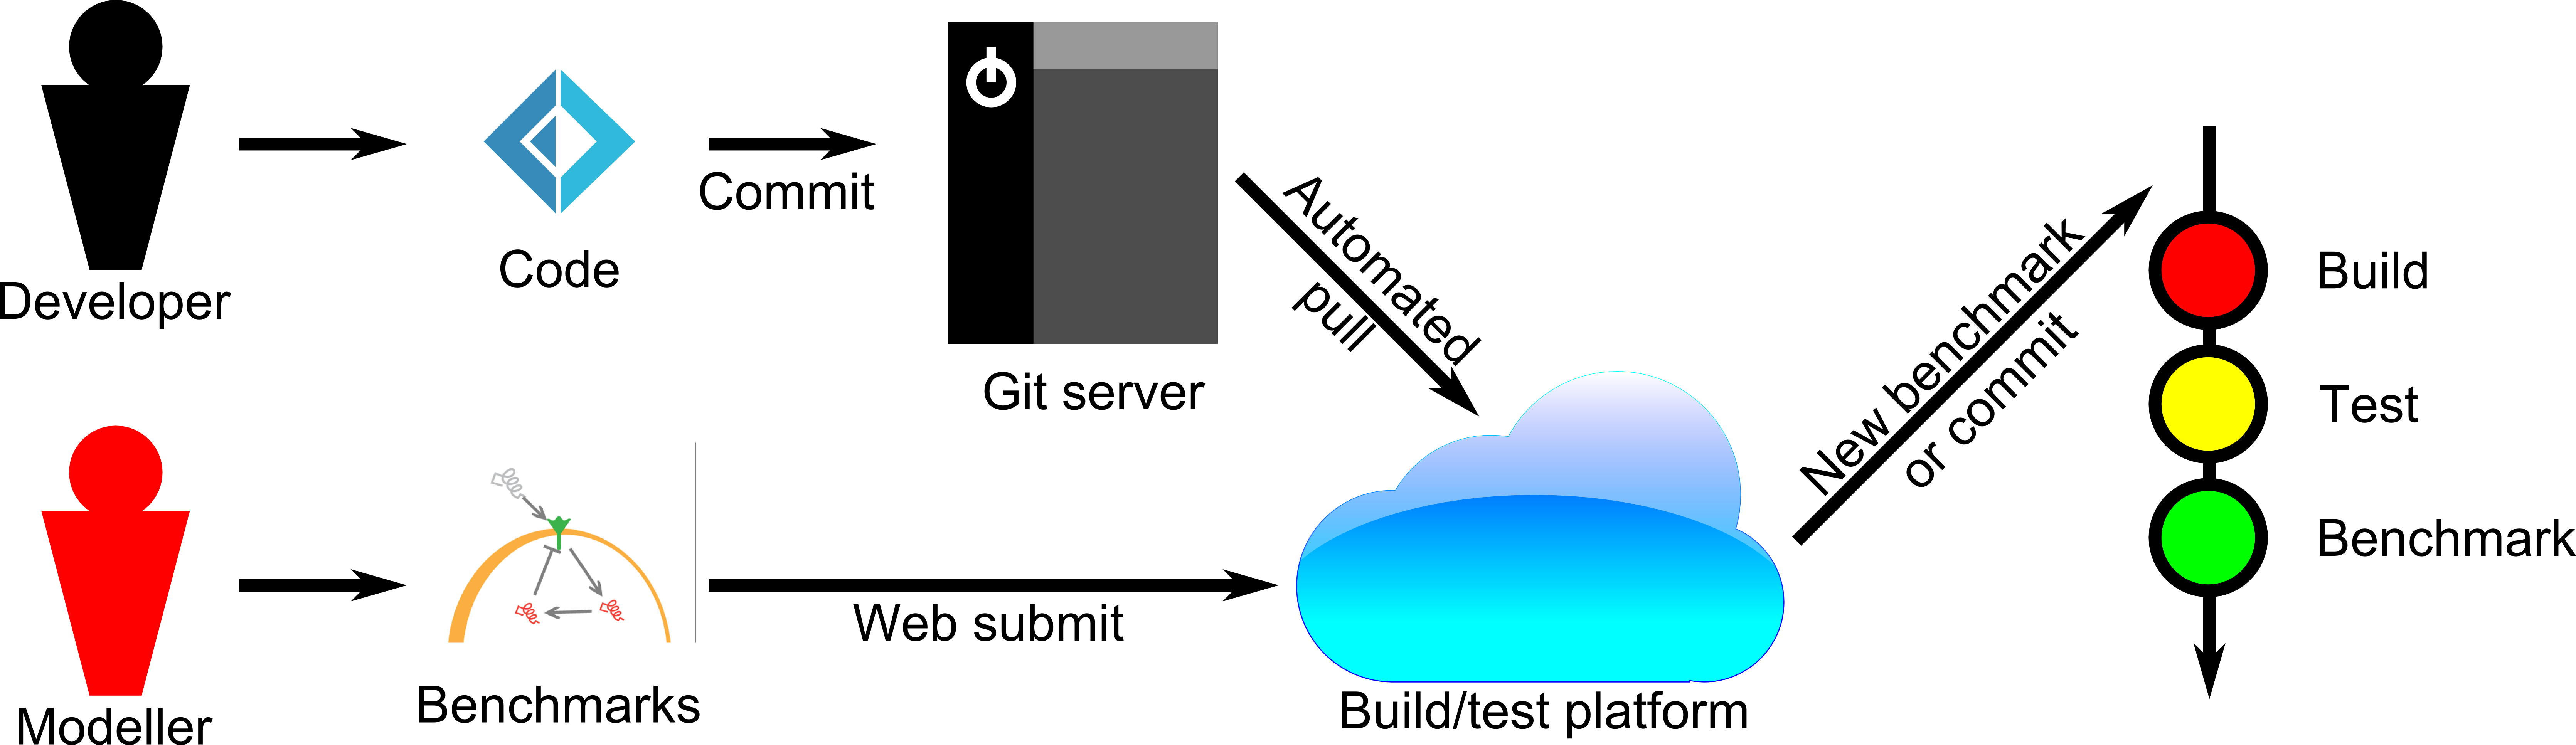
\includegraphics[width=\textwidth]{workflow}
	\caption{Proposed reproducibility service workflow}
	\label{schematic}
\end{figure}
	
To address these needs we propose that the service should follow the
scheme given in Figure~\ref{schematic}. Two classes of user are
defined; developers, who generate code, and modellers, who generate
new benchmarks. An individual might in practice play either or both of
these roles; here the roles serve to define ways in which people
interact with the system. A developer writes new code, which is
periodically pushed to a repository such as GitHub. Through
integration with the repository, the server responds to new code by
undergoing a process of pulling the code from the repository,
downloading required dependencies, and compiling the code. If this
stage fails, the developer is informed and the workflow ends. If the
code is successfully compiled, two stages of testing are
performed. The first stage (labelled {\emph{test}} in
Figure~\ref{schematic}), involves running a series of basic tests
defined by the developer. This is intended as a sanity check to ensure
that basic features of the code have not been broken by the updated
code, and failure to pass these tests is reported and ends the work
flow. If this completes successfully, the second stage (labelled
{\emph{benchmark}} in Figure~\ref{schematic}) a series of models are
tested for a known property, and the results recorded. These results
can then be stored in a database, with a note of the commit ID, and
available through a web interface for future analysis.

In contrast to the developer role, a modeller supplies benchmarks for
a piece of code to test. These do not require that the latest version
of the code is recompiled, but on submission the models are tested and
added to the local repository of models for analysis. After a model is
submitted, the model is tested on every new piece of code pushed to
the server and the changes in the behaviour can be noted and linked to
specific code commits. Whilst the developers role has a transparent
value (in providing an implementation of an algorithm), the value of
the modeller may be less immediately clear. The modeller submits a
broad range of tests which may highlight material flaws (i.e. bugs) in
the implementation, or the algorithm. More than this however, the
modeller may generate models which identify weaknesses of either an
algorithm or an implementation. One example from the authors
experience is the series of models with ``timed-switches'' described
in \cite{cook2014}; this is discussed in greater depth below in
section~\ref{example}.

Finally, dependencies for a given implementation need explicit
testing. Due to the highly variable and sometimes complex nature of
dependencies, we see this as an optional part of the workflow, as
developers may chose to supply dependencies as binary files in the
code compilation process. For completeness however we note that such a
system could also respond to updates in external dependencies by
triggering compilation and testing in the same manner as defined for a
new code commit. This would aid developers in identifying code
breaking changes induced by third parties.


%\section{Introducing reproducibility testing to the community}\label{rollout}
\section{A reproducibility model for the CAV community}\label{rollout}

Following the proposal of such a system, the question becomes:
{\emph{how do we encourage widespread uptake, or even standardisation?}}
Such a service may appear trivial, given the large numbers of tools
which could potentially support the service. There remain however key
questions that can only be answered on implementation. Furthermore,
after such a service has been implemented, how do we ensure it is
\emph{useful} and \emph{usable} for researchers.

% workflow

\begin{enumerate}
\item Call for papers: clearly advertised and high profile in conf cfp
  -- this is a new thing and a change in how we're doing stuff.
\item The game is changing, but this is (currently) extra to the
  normal reviewing process: 
e.g. {\emph{This submission is voluntary and will not influence the final decision
regarding the papers.}} -- independent of the scientific merit of the
paper, the results will be verified 
\item (prize? as well as ranked ordering at end of conf, listed in
  proceedings, badge, seal of approval, etc)
\item explicit criteria for authors? but essentially: {\emph{make this
      as easy as possible for us to evaluate/execute your artefact!}}
\item when papers are submitted, they have to nominate whether they
  want their paper to go through artefact review
\item (then you need artefact reviewers, probably taken from the pool of
  reviewers, but will need specialism)
\item specify review criteria, but essentially: {\emph{can I evaluate/execute this
  artefact and get the same results that are presented in the paper?}}
\item reporting: traffic lights and ranked list
\item at the start, this is not compulsory, but this will change over a period of
time -- effecting cultural change and this would then become a
necessary condition.
\item Repo/database or previous artefacts, which would build over the
  years to give exemplars and comparisons.
\end{enumerate}

The key question for different research communities then becomes: how
to initialise this change? Such a requirement creates a set of new
costs to researchers, both in terms of time spent ensuring that their
tools work on the centralised system (in addition to their local
implementation), but also potentially in terms of equipment (in terms
of running the system). Such costs may be easier to bear for some
groups compared to others, especially those with large groups who can
more easily distribute the tasks, and it is important that the service
does not present a barrier to early career researchers and those with
efficient budgets. This type of cost is not unique to reproducibility
efforts- it has been estimated (in CACM, a closed but arguably
affordable journal) that a shift to becoming exclusively open access
may lead to a ten-fold increase in computer science publication
costs~\cite{vardi-cacm-2014}. 

\section{Example case study: BioModelAnalyzer}\label{example}

% NEEDS WORK!
% IDEA: pick one of Samin's CAV papers (BMA?) and run it through the
% process and see what happens.

The
BioModelAnalyzer\footnote{\url{http://biomodelanalyzer.research.microsoft.com/}}
is a tool for the development and analysis of a specific class of
formal models for
biology~\cite{benque2012,cook-et-al:2010,cook2014}. Models are built
by biologists in a web browser and are explored at present by a
combination of simulation and model checking. The tool specifically
allows users to test for model \emph{stability}; that is, a bespoke
algorithm proves that for all initial states a model always ends in a
single fixpoint. We have chosen this example due to our familiarity
with the tool, and to highlight historical examples where a
reproducibility service would have supported both code development and
algorithm discovery.

Suggested things to discuss here- the proposed benefits of such a service:

Local hacks to publish are not communicated preventing reuse
(specific commands required to compile and publish the code, 
relating to 64- and 32- bit capabilities, were not distributed
and lost when a team member left)
Service would- highlight when a codebase could not be compiled or run

Effects of rounding mechanisms in the algorithm implementation
(swapping floors and rounds broke some things subtly)
Service would- highlight these changes in behaviour clearly

Impact of implementing "biological" intuition in the tool
(changing the default target function of nodes with no inputs, also
breaking things subtly)
Service would- highlight the problems created

Modelling reveals untested issues: range conversion
(no original benchmarks had range conversion- new benchmarks did
and showed unexpected behaviour, including a mismatch between symbolic
and explicit implementations of range conversion)
Service would- allow external users to add new benchmarks, which would make it
easier to catch these issues

Modelling reveals algorithmic weakness: timed switch models 
(a new class of models was discovered which forced the tool to search 
for large cycles explicitly to prove stability)
Service would- allow these new models to have been identified earlier
by highlighting that proofs of stability consistently timed out
Service would- make it easier to prove stability multiple ways (e.g.
through the LTL checker of CAV13)
Service would- show the improvement in speed resulting from the introduction
of the new algorithm

% Worked example of how issues could be highlighted and found over time: perhaps
% another figure? linking code changes to discoveries could be drawn as a timeline. The 
% proposed output of the hypothetical service could be indicated alongside it, 
% demonstrating how the service would have supported the work.

% should this be merged into the section above? Cite Fursin et al.
% Problem: getting people to do it? Carrot/stick...
\section{Known unknowns: issues for a reproducibility service}\label{issues} 

How to effectively ``generalise'' for reuse and then cascading to other communities?

How best to secure a service which compiles and runs arbitrary code on arbitrary inputs?

How to estimate raw performance on the cloud?

\section{Conclusions}\label{concl}
We thus propose that this could be trialled for CAV in 2016, with a
announced schedule for widespread adoption in future years...

The benefits to the community from a cultural change to favour
reproducibility are clear however, and as such we should aim through
the software and the roll-out to mitigate these costs. Furthermore, we
can reasonably expect the needs of the community to evolve over time,
and initial implementations of the platform may require refinement in
response to user feedback. As such, if the community is to move to
requiring reproducibility, it seems most reasonable that this is
staggered over a number of years to allow for both of these elements
to develop. We recommend that the tools pass through two testing
phases, until eventually all authors are required to use the service.

\begin{description}
\item[Phase 1:] Offer the service as an optional extra in the testing phase, allowing users to demonstrate 
the reliability of their code which could be taken into account in the review process.
\item[Phase 2:] All authors must use the reproducibility service, but results are not used in the review
process. The results of the test are used to refine the service and pick out any unaddressed issues
\item[Phase 3:] All authors are required to use the service, and the results are explicitly used to 
assess reproducibility in the review process.
\end{description}

This plan balances competing needs within the community, and would reduce the activation
energy for uptake by gradually introducing it to authors.

\bibliographystyle{splncs}
\bibliography{cav2015}

\end{document}
